\documentclass[14pt, professionalfont]{article}

\usepackage{amssymb, amsfonts, amsthm}
\usepackage[fleqn]{amsmath}
\usepackage[dvipsnames]{xcolor}
\usepackage[many]{tcolorbox}
\usepackage{fancyhdr}
\usepackage{atbegshi}
\usepackage[hidelinks]{hyperref}
\usepackage{float}
\usepackage[left=0.18\paperwidth, right=0.18\paperwidth, top=0.12\paperheight, bottom=0.18\paperheight]{geometry}


\usepackage{graphicx}
\usepackage{framed}

\usepackage[perpage]{footmisc}
\usepackage{wrapfig}
\usepackage{subcaption}
\usepackage{booktabs}
\usepackage{tabu}

\usepackage{xepersian}
\settextfont{IRLotus}
\setdigitfont{IRLotus}
\setlatintextfont{Tom's New Roman}

\renewcommand{\baselinestretch}{1.15} 
\setlength{\mathindent}{0pt}
\setcounter{secnumdepth}{4}
\setcounter{tocdepth}{4}
\hypersetup{
	colorlinks=false,
	pdfborder={0 0 0},
}

\title{ پروژه۳ سیستم های مخابرات 
	}
\author{دکتر صباغیان}
\date{نیم سال اول 98-99 }

\makeatletter
\let\thetitle\@title
\let\theauthor\@author
\let\thedate\@date
\makeatother

\pagestyle{fancy}
\fancyhf{}
\rhead{\theauthor}
\lhead{\thetitle}
\cfoot{\thepage}

\newcommand{\E}{\text{$\mathbb{E}$}}
\renewcommand{\P}{\text{$\mathbb{P}$}}

\begin{document}	
	\begin{titlepage}
		\centering
		\vspace*{2 cm}
		\begin{minipage}{\textwidth}
			\begin{minipage}{0.5\textwidth}
				\flushright
				
\includegraphics[scale = 0.55]{ece.png}
				\vspace*{0.5 cm}
			\end{minipage}
		\begin{minipage}{0.5\textwidth}
			\flushleft
			
\includegraphics[scale = 0.30]{ut.png}
			\vspace*{0.5 cm}
		\end{minipage}		
	\end{minipage}

		\textsc{\LARGE دانشکده فنی دانشگاه تهران}\\[0.5 cm]
		\textsc{\Large دانشکده برق و کامپیوتر}\\[0.5 cm]
		\rule{\linewidth}{0.2 mm}
		{ \LARGE \bfseries \thetitle}\\
		\vspace{4pt}
			\lr{Digital Modulation}
		
		\rule{\linewidth}{0.2 mm} \\[1.5 cm]
		\begin{minipage}{0.2\textwidth}
			\begin{flushright} \large
				\emph{طراح:}\\
				\rl{سجاد پاکدامن ساوجی}
				
			\end{flushright}
		\end{minipage}~
		\begin{minipage}{0.3\textwidth}
			\begin{flushleft} \large
				\emph{رایانامه} \\
				\lr{sj.pakdaman@ut.ac.ir}
			\end{flushleft}
		\end{minipage}\\[2 cm]
		{\large \thedate}\\[2 cm]
		\vfill
	\end{titlepage}

	{ \Large
		
		دانشجویان عزیز، قبل از پاسخ‌گوئی به سوالات به نکات زیر توجه کنید:
		\begin{enumerate}
			\item 
			شما باید کدها و گزارش خود را با الگو
			\:
			\lr{CA3\_StudentNumber.zip}
			\:
			در محل تعیین شده آپلود کنید
			\item 
			گزارش کار شما نیز جزو معیار های ارزیابی خواهد بود در نتیجه زمان کافی	 برای تکمیل آن اختصاص دهید
			\item 
			
			قسمت اصلی کد شما باید در محیط 
			\:
			\lr{matlab live editor}
			\:
			نوشته شود و نمودار ها علاوه‌ بر گزارش کار باید در کد اصلی نیز قرار داشته باشند

			\item 
			شما میتوانید سوالات خود را از طریق ایمیل
			\textcolor{blue}{
				\: 
				\href{mailto:sj.pakdaman@ut.ac.ir}{sj.pakdaman@ut.ac.ir}
				\:}
			بپرسید
		\end{enumerate}
	}
	
	\thispagestyle{empty}
	\clearpage
	\pagenumbering{arabic} 
	\pagebreak
	در این تمرین کامپیوتری به شبیه سازی کانال 
	\:
	\lr{AWGN}
	\:
	می‌پردازیم و با استفاده از روش های تخمین چگالی غیر‌پارامتری چگالی خروجی کانال را تخمین می‌زنیم. در پایان تابع احتمال خطا برای مدولاسیون دیجیتال 
	\:
	\lr{PCM}
	\:
	را به صورت تئوری و عددی محاسبه می‌کنیم و شرایط هم‌گرایی دو تابع احتمال خطا را بررسی می‌کنیم.
	
	
	\begin{enumerate}
		\item 
		ساده ترین روش برای تخمین چگالی احتمال استفاده از روش غیر پارامتری هیستوگرام است. این نوع تخمین دارای دو هایپر‌ پارامتر است ،‌تعداد داده ها
		\:
		$N$
		\:
		و تعداد بخش‌هایی که داده ها در آن تقسیم‌ می‌شوند
		\:
		\lr{bins}
		\:
		. برای این که تخمین هیستوگرام به تابع چگالی احتمال همگرا شود باید شرایط زیر برقرار باشد.
		$$
		N \rightarrow \infty \qquad bins \rightarrow \infty \qquad such \: that \quad \frac{N}{bins} \rightarrow \infty
		$$
		در این قسمت می‌خواهیم تابع چگالی احتمال گوسی را برای تمرین تخمین بزنیم و با تغییر پارامتر های 
		\:
		$\mu$
		\:
		و 
		\: 
		$\sigma$
		\:
		نحوه تغییر چگالی را مشاهده کنیم. با استفاده از تابع 
		\:
		\lr{normrnd()}
		\:
		به تعداد 
		\:
		$N$
		\:
		داده رندوم از تابع چگالی گوسی با 
		\:
		$\mu = 0 $
		\:
		و 
		\:
		$\sigma = 1$
		\:
		تولید کنید و سپس تابع چگالی را با با هیستوگرام با 
		\:
		\lr{bins}
		\:
		تقریب بزنید. پارامتر های 
			\:
		$N$
		\:
		و
		\:
		\lr{bins}
		\:
		را بگونه ای انتخاب کنید که تابع چگالی شکل نرمی داشته باشد. برای رسم هیستوگرام می‌توانید از تابع
			\:
		\lr{hist()}
		\:
		استفاده کنید. دقت کنید که توابعی که تولید اعداد تصادفی می‌کنند در حقیقت اعداد شبه‌تصادفی تولید می‌کنند به این معنی که برای تولید اعداد از یک عدد ثابت به عنوان 
		\:
		\lr{seed}
		\:
		استفاده می‌کنند. در نرم افزار متلب تابعی که تولید اعداد تصادفی را مدیریت می‌کند 
		\:
		\lr{rng}
		\:
		نام دارد. قبل از تولید اعداد تصادفی باید از دستور 
		\:
		\lr{rng shuffle}
		\:
		استفاده کنید تا اعداد تولید شده تکرار نشوند.
		
		تابع چگالی گوسی را با پارامتر های 
		\:
		$\mu = 0$
		\:
		و 
		\:
		$\sigma = \{1,2,3\}$
		\:
		تقریب بزنید. 
		
	
		
		
				\begin{figure}[h]
				\centering
				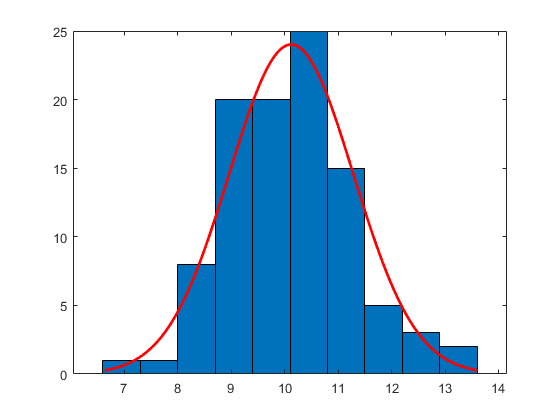
\includegraphics[scale = 0.25]{../images/hist.png}
				\caption{
					تخمین چگالی با استفاده از 
					\lr{histogram}
				}
			\end{figure}
		
		\item 
		در فرایند اثبات احتمال خطای کانال 
		\:
		\lr{AWGN}
		\:
		دیدید که اگر چگالی گوسی با یک عدد ثابت جمع شود ،‌ میانگین آن چگالی تغییر می‌کند.تابع چگالی احتمال متغیر‌های تصادفی 
		\:
		$X \sim norm(5,1)$
		\:
		و
		\: 
		$Y \sim  norm(0,1) + 5$
		\:
		را با استفاده از هیستوگرام تخمین بزنید. با نوشتن روابط ریاضی مربوط به امید‌ریاضی این دو متغیر تصادفی اثبات کنید که میانگین آن‌ها یکی است.
		
	
	\item 
	در این قسمت می‌خواهیم شبیه سازی اولیه‌ای از کانال 
	\:
	\lr{AWGN}
	\:
	انجام دهیم. فرض کنید که از کانال با مدولاسیون 
	\:
	\lr{PCM}
	\:
	استفاده می‌کنیم به این صورت که با احتمال 
	\:
	$p_1 = \frac{1}{2}$
	\:
	عدد 
	\:
	$+1$
	\:
	و با احتمال 
	\:
	$p_2 = \frac{1}{2}$
	\:
	عدد 
	\:
	$-1$
	\:
	را می‌فرستیم. برای انجام این شبیه سازی شما باید تعداد زیادی پیام را از کانال عبور دهید تا شرایط هم‌گرایی تخمین هیستوگرام برقرار شود. برای انتخاب با احتمال های 
	\:
	$p_1$
	\:
	و 
	\:
	$p_2$
	\:
	از بین اعداد 
	\:
	$+1$
	\:
	و 
	\:
	$-1$
	\:
	می‌توانید تابعی بر‌اساس دستور 
	\:
	\lr{rand()}
	\:
	پیاده‌سازی کنید.  با توجه به کانال شکل ۲ تابع چگالی احتمال خروجی کانال را تخمین بزنید.
	
		\begin{minipage}[c]{0.45\textwidth}
		\begin{figure}[H]
			\centering
			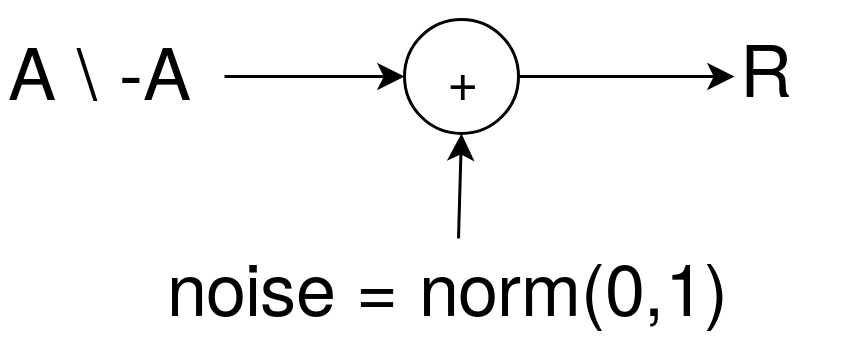
\includegraphics[scale = 0.18]{../images/diagram.png}
			\caption{
				کانال 
				\:
				\lr{AWGN}
			}
		\end{figure}
	\end{minipage}
	\begin{minipage}[c]{0.5\textwidth}
		\begin{figure}[H]
		\centering
		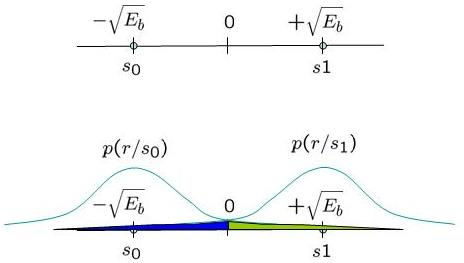
\includegraphics[scale = 0.35]{../images/awgn.jpg}
		\caption{چگالی احتمال خروجی کانال
			\:
			\lr{AWGN}
		}
	\end{figure}
	\end{minipage}
\item 
تخمین قسمت قبل را برای 
\:
$p_1 = 0.3$
\:
 و 
 \: $p_2 = 0.7$
 \:
 مجددا انجام دهید. در حالتی که احتمال های برابر هستند مرز تصمیم گیری عدد ۰ می‌باشد. آیا پس از تغییر احتمال های 
 \:
 $p_1$
 \:
 و 
 \: $p_2$
 \:
 مرز تصمیم گیری همچنان ۰ باقی می‌ماند؟
 \item 
 در این قسمت می‌خواهیم نمودار های احتمال خطا کانال 
 \:
 \lr{AWGN}
 \:
 با نویز جمع‌ شونده 
 \:
 $n \sim normal(0,1)$
 \:
 و احتمال های ارسال برابر 
 \:
 $p_1 = p_2 = 0.5$
 \:
 به صورت تئور و عددی بدست آوریم.
 $$
 p_e = Q\left(\frac{A}{\sqrt{N_R}}\right)=Q\left(\frac{\sqrt{S_R}}{\sqrt{N_R}}\right) = 
 Q\left(\sqrt{\left(\frac{S}{N}\right)_R}\right)
 $$
	برای محاسبه عددی احتمال خطا در یک 
	\:
	$\left(\frac{S}{N}\right)_R$
	\:
	مشخص باید تعداد زیادی 
	\:
	$\pm 1$
	\:
	با آن 
	\:
	$\left(\frac{S}{N}\right)_R$
	\:
	خاص از کانال عبور داده شود و در سمت خروجی کانال تشخیص داده شود که هر پیام 
	\:
	$+1$
	\: 
	بوده است یا
	\:
	$-1$
	\:
	، سپس با تقسیم تعداد تشخیص های درست به کل پیام های ارسال شده احتمال خطا ذر آن 
	\:
	$\left(\frac{S}{N}\right)_R$
	\:
	بدست می‌آید. برای تشخیص 
	\:
	$+1$
	\:
	یا
	\:
	$-1$
	\:
	بودن یک پیام از مرز تصمیم ۰ استفاده کنید ،‌به این صورت که اگر در خروجی عدد بزرگ‌تر از ۰ باشد 
	\:
	$+1$
	\:
	تشخیص داده می‌شود و اگر عدد در خروجی کوچکتر از ۰ باشد 
	\:
	$-1$
	\:
	تشخیص داده می‌شود.
	
	نمودار های تئوری و عددی احتمال خطا کانال 
	\:
	$p_e$
	\:
	در مقیاس 
	\:
	$dB$
	\:
	بر حسب 
	\:
		$\left(\frac{S}{N}\right)_R \epsilon [0,4]$
	\:
	در یک نمودار رسم نمایید. تعداد ارسال ها برای هر
	\:
	$\left(\frac{S}{N}\right)_R$
	\:
	خاص را آن قدر افزایش دهید تا دو نمودار هم‌گرا شوند .
		\begin{figure}[H]
		\centering
		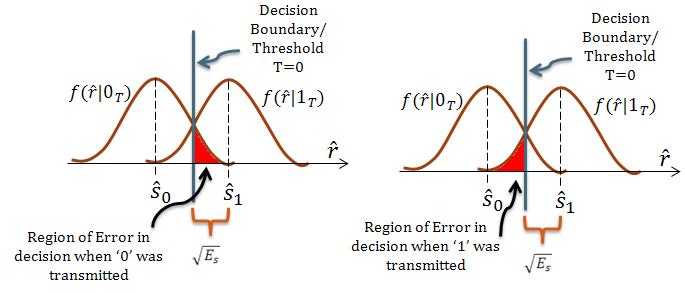
\includegraphics[scale = 0.35]{../images/error.png}
		\caption{
			ایجاد خطا در گیرنده در کانال
			\:
			\lr{AWGN}
		}
	\end{figure}
	
	\end{enumerate}
\end{document}